\section{Analysis}

We analyze \ours{} through several aspects: incorporating failure trajectories, examining emergent strategies, and evaluating efficiency across both successful and failed cases. Additional analyses are presented in Appendix~\ref{app: analysis}, including but not limited to number of retrieved experiences, additional results on smaller open-source model, and inference cost study.

\begin{figure}[t]
\begin{center}
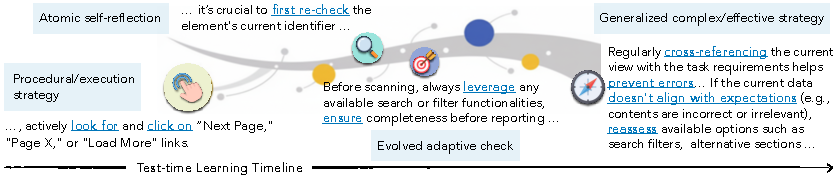
\includegraphics[width=\textwidth]{figures/evolving_strategy.pdf}
\end{center}
\vspace{-3mm}
\caption{A case study illustrating emergent behaviors in \ours{} through memory items.}
\vspace{-5mm}
\label{fig: evolving_strategy}
\end{figure}

\begin{wrapfigure}{r}{0.38\textwidth}
% \vspace{-5mm}
  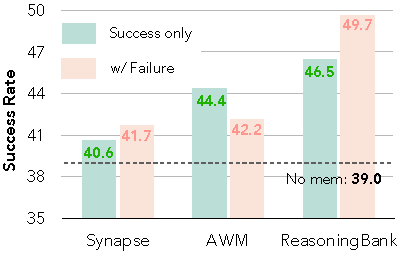
\includegraphics[width=0.38\textwidth]{figures/ablation_failure.pdf}
  \vspace{-5mm}
  \caption{Ablation results of incorporating failure trajectories for memory induction.}
  \label{fig: ablation_failure}
  \vspace{-3mm}
\end{wrapfigure}

\paragraph{Emergent behaviors with \ours{}.}~\label{exp: emergent}
We find that the strategies in \ours{} are not flat or monolithic, but instead evolve over time, exhibiting emergent behaviors that resemble the learning dynamics of RL~\citep{wang2025emergent}. As illustrated in a human case study in Figure~\ref{fig: evolving_strategy}, memory items describing a specific strategy ``\textit{User-Specific Information Navigation}'' in \ours{} could gradually evolve during test-time learning process. It starts from execution-oriented or procedural strategies (e.g., find navigation links), where the agent follows straightforward action rules. It then progresses to adaptive self-reflections such as re-verifying identifiers to reduce simple mistakes. With more experiences, the same memory item evolves into adaptive checks, where the agent systematically leverages available search or filters to ensure completeness before results. Finally, it eventually matures into compositional strategies such as cross-referencing task requirements and reassessing options. This evolution highlights how \ours{} enables agents to refine strategies from low-level actions to high-level reasoning during test-time learning.



\paragraph{\ours{} makes good use of failure trajectories.}~\label{exp: ablation}

Figure~\ref{fig: ablation_failure} compares different memory designs on WebArena-Shopping with Gemini-2.5-flash under two settings: using only successful trajectories versus leveraging both successes and failures. 
Baseline methods such as Synapse and AWM build memory solely from successful trajectories, and thus are not equipped to benefit from failures. 
As a result, when failures are added, their performance is limited or even degraded: Synapse increases only from $40.6$ (success only) to $41.7$ (with failures), while AWM drops from $44.4$ to $42.2$. 
In contrast, the design of \ours{} enables distillation of reasoning patterns from \emph{both} successes and failures, achieving $46.5$ on success-only traces and further improving to $49.7$ when failures are included. 
This highlights that, unlike baselines, \ours{} can transform failures into constructive signals rather than noise, enabling more robust generalization.


\paragraph{\ours{} exhibits robustness to LLM-as-a-Judge calibration.}
\begin{wrapfigure}{r}{0.38\textwidth}
\vspace{-5mm}
  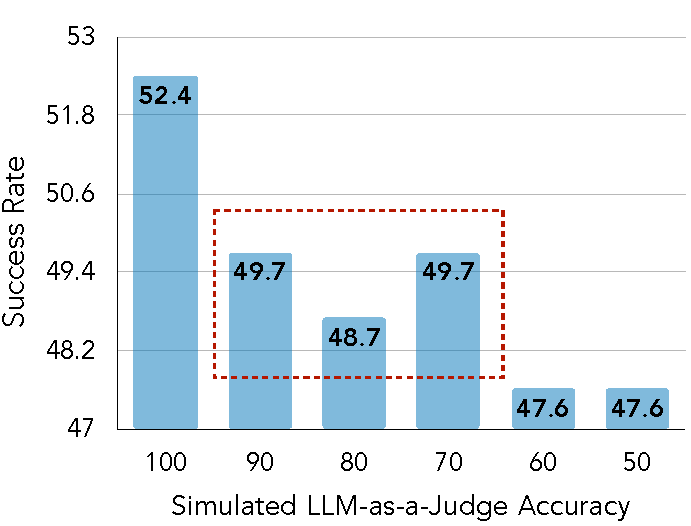
\includegraphics[width=0.38\textwidth]{figures/judge_accuracy.pdf}
  \vspace{-5mm}
  \caption{Results for SR w.r.t. simulated LLM-as-a-judge accuracy.}
  \label{fig: judge_accuracy}
  \vspace{-3mm}
\end{wrapfigure}
A critical step in our method is sourcing proxy correctness signals for agent trajectories via an LLM-as-a-Judge. Here we quantitatively calibrate this judge and analyze its robustness to verification noise. We conduct our analysis on the WebArena-Shopping subset, using Gemini-2.5-flash as the judge. We first establish the baseline accuracy by comparing the judge's predictions against ground-truth labels, which we find to be 72.7\%.
To systematically study the robustness of \ours{} to the judge quality, we simulate different levels of verification accuracy. This is achieved by probabilistically correlating the judge's labels with the ground-truth. For example, a 100\% accurate verifier uses the ground-truth labels directly. A 90\% accurate verifier is simulated by using the correct (ground-truth) label 90\% of the time and the incorrect (flipped) label 10\% of the time. We extend this simulation down to 50\% accuracy, which represents a random-guess baseline for this binary (success/failure) classification task. The results are presented in Figure~\ref{fig: judge_accuracy}.
We observe that the judge's accuracy does not significantly impact the performance of \ours, as all variants achieve similar success rates within reasonable accuracy range (70\%-90\%). Intuitively, the 100\% (ground-truth) accuracy setting yields the best performance. These findings confirm that \ours is robust to noise in the verification step.



\paragraph{\ours{} delivers targeted efficient gains.}~\label{exp: efficiency}
\begin{table}[!t]
\centering\setlength{\tabcolsep}{3.5pt}
\small
\setlength{\belowcaptionskip}{5pt}
  \caption{Average number of steps on successful and failed test instances across four WebArena domains. \ours{} consistently reduces the number of steps compared to the vanilla baseline, with notably larger reductions on successful instances.}
  \label{table: steps}
  \begin{tabular}{lcccccccc}
    \toprule
    \multirow{2}{*}{\textbf{Models}} &\multicolumn{2}{c}{\textbf{Shopping}}&\multicolumn{2}{c}{\textbf{Admin}}&\multicolumn{2}{c}{\textbf{Gitlab}}&\multicolumn{2}{c}{\textbf{Reddit}}\\
\cmidrule(lr){2-3}\cmidrule(lr){4-5}\cmidrule(lr){6-7}\cmidrule(lr){8-9}
&\textit{Successful}&\textit{Failed}&\textit{Successful}&\textit{Failed}&\textit{Successful}&\textit{Failed}&\textit{Successful}&\textit{Failed} \\
    \midrule
    No Memory &6.8&8.7&8.4&10.4&8.6&15.7&6.1&7.6\\
    \ours{} &4.7\uag{$\downarrow$2.1}&7.3\uag{$\downarrow$1.4}&7.0\uag{$\downarrow$1.4}&9.5\uag{$\downarrow$0.9}&7.6\uag{$\downarrow$1.0}&15.5\uag{$\downarrow$0.2}&5.0\uag{$\downarrow$1.1}&6.8\uag{$\downarrow$0.8} \\

  \bottomrule
\end{tabular}
\vspace{-3mm}
\end{table}

While the overall number of steps in Table~\ref{table: webarena} provides a general view of model efficiency, it does not distinguish whether reductions come from successful or failed trajectories. To gain deeper insight, we further separate the analysis into successful and failed  test cases, which allows us to understand the source of step reduction: 
a desirable system should reduce unnecessary exploration when it is on the right track, rather than merely cutting short failed attempts. 
The results are shown in Table~\ref{table: steps}. We find that \ours{} consistently reduces the number of steps across all domains compared to the baseline. More importantly, the reduction is particularly pronounced on successful cases, reaching up to $2.1$ fewer steps (a $26.9\%$ relative reduction) than on failed ones. This indicates that \ours{} primarily helps the agent reach solutions with fewer interactions by strengthening its ability to follow effective reasoning paths rather than simply truncating failed trajectories, which highlight the role of memory in guiding purposeful decision-making and improving efficiency in practice.